\chapter{Specifikacija programske potpore}
		
\section{Funkcionalni zahtjevi}

\noindent \textbf{Dionici:}
			
\begin{packed_enum}
	
	\item Vlasnik (naručitelj)
	\item Učenici				
	\item Administratori
	\item Razvojni tim
	
	
\end{packed_enum}

\noindent \textbf{Aktori i njihovi funkcionalni zahtjevi:}
			
			
\begin{packed_enum}
	\item  \underbar{Administrator (inicijator) može:}
	
	\begin{packed_enum}
		
		\item pregledati i odabrati jezik te unutar tog jezika
		\begin{packed_enum}
			
			\item stvoriti, urediti, brisati i pregledati riječi (riječ, opis, fraze, prijevod)
			\item stvoriti, urediti, brisati i pregledati rječnike (naziv, broj riječi)
			\item dodati ili ukloniti riječ/i iz jednog ili više rječnika
			\item stvoriti administratore 
			\item brisati administratore
	
		\end{packed_enum}
		
	\end{packed_enum}

	\item \underbar{Učenik (inicijator) može:}
	
	\begin{packed_enum}

		\item pregledati i odabrati dostupne jezike
		\item pregledati i odabrati dostupne rječnike odabranog jezika
		\item započeti učenje odabirom jednog od četiri načina učenja
		\item izbrisati svoj korisnički račun 
	
	\end{packed_enum}

	\item  \underbar{Baza podataka (sudionik) može:}
	
	\begin{packed_enum}
		
		\item pohraniti sve podatke o učenicima i njihovim (ne)naučenim riječima
		\item pohraniti sve podatke o učenicima o administratorima 
		\item pohraniti sve podatke o riječima i rječnicima
		
	\end{packed_enum}

	\item  \underbar{API za rječnike (sudionik) može:}
	
	\begin{packed_enum}
		
		\item dohvatiti dodatne podatke o riječima (opis, fraza)
		
	\end{packed_enum}

	\item	\underbar{Neregistrirani korisnik (inicijator) može:}
	
	\begin{packed_enum}
		
		\item registrirati se:
		
		\begin{packed_enum}		
			
			\item potvrditi registraciju prijavom s inicijalnom lozinkom
			\item promijeniti inicijalnu lozinku
		
		\end{packed_enum}

	\end{packed_enum}

	\item	\underbar{Servis za ocjenu izgovora (sudionik) može:}
	
	\begin{packed_enum}
		
		\item ocijeniti korisnikov izgovor neke riječi ili izraza

	\end{packed_enum}

	\item	\underbar{Davatelj e-pošte (sudionik) može:}
	
	\begin{packed_enum}
		
		\item pruža uslugu stvaranja i korištenja e-mail računa

	\end{packed_enum}

\end{packed_enum}

\eject

\subsection{Obrasci uporabe}

\subsubsection{Opis obrazaca uporabe}


\noindent \underbar{\textbf{UC1 - Registracija}}
\begin{packed_item}

	\item \textbf{Glavni sudionik:} Neregistrirani korisnik
	\item  \textbf{Cilj:} Stvaranje učeničkog računa
	\item  \textbf{Sudionici:} Baza podataka, davatelj e-pošte
	\item  \textbf{Preduvjet:} Učenik nije registriran niti prijavljen u sustav
	\item  \textbf{Opis osnovnog tijeka:}
	
	\item[] \begin{packed_enum}

		\item Korisnik odabire opciju ”Registracija”
		\item Korisnik unosi ime, prezime, e-mail i potvrđuje prijavu
		\item Korisnik na svoj e-mail dobiva privremenu generiranu lozinku
		\item Korisnik se prijavljuje u sustav s generiranom lozinkom (UC3 Prijava u sustav)							
		\item Sustav učeniku prikazuje obrazac za promjenu inicijalne lozinke (nastavak UC2 Promjena lozinke)
	\end{packed_enum}
	
	\item  \textbf{Opis mogućih odstupanja:}
	
	\item[] \begin{packed_item}

		\item[2.a]Korisnik se pokušava registrirati e-mail adresom na koju je već prijavljen račun
		\item[] \begin{packed_enum}
			
			\item Sustav upozorava korisnika i onemogućuje mu registraciju							
		\end{packed_enum}

	\end{packed_item}

\end{packed_item}

\noindent \underbar{\textbf{UC2 - Promjena lozinke}}
\begin{packed_item}

	\item \textbf{Glavni sudionik:} Učenik
	\item  \textbf{Cilj:} promjena lozinke
	\item  \textbf{Sudionici:} Baza podataka
	\item  \textbf{Preduvjet:} UC1 Registracija 
	\item  \textbf{Opis osnovnog tijeka:}
	
	\item[] \begin{packed_enum}

		\item Učenik u postavkama svog računa bira opciju "Promjena lozinke"
		\item Učeniku se prikazuje dijaloški okvir u kojem treba unijeti i potvrditi svoju novu lozinku
		\item Sustav preusmjerava korisnika na zaslon za odabir jezika (UC7 Pregledavanje i odabir jezika)
	\end{packed_enum}
	
	\item  \textbf{Opis mogućih odstupanja:}
	
	\item[] \begin{packed_item}

		\item[1.a]Učenik gasi aplikaciju
		\item[] \begin{packed_enum}
			
			\item Ne dolazi do promjene lozinke, učenik mora ponoviti proces					
		\end{packed_enum}

		\item[2.a]Polja "lozinka" i "potvrdi lozinku" se razlikuju
		\item[] \begin{packed_enum}
			
			\item Sustav upozorava učenika i traži ispravak unosa			
		\end{packed_enum}
		
	\end{packed_item}
\end{packed_item}


\noindent \underbar{\textbf{UC3 - Prijava u sustav}}
\begin{packed_item}

	\item \textbf{Glavni sudionik: } Učenik ili administrator
	\item \textbf{Cilj: } Dobivanje pristupa učeničkom ili administratorskom sučelju
	\item \textbf{Sudionici: } Baza podataka
	\item \textbf{Preduvjet: } -
	\item  \textbf{Opis osnovnog tijeka:}
	
	\item[] \begin{packed_enum}

		\item Korisnik aplikacije unosi svoj e-mail i lozinku
		\item Sustav provjerava postoji li račun s istim podacima
		\item Ako su podaci ispravni, sustav preusmjerava korisnika na zaslon za odabir jezika (nastavak UC7 Pregledavanje i odabir jezika)

	\end{packed_enum}
	
	\item  \textbf{Opis mogućih odstupanja:}
	
	\item[] \begin{packed_item}

		\item[2.a] Neispravan e-mail ili lozinka
		\item[] \begin{packed_enum}
			
			\item Sustav obavještava korisnika o grešci
			
		\end{packed_enum}
		
	\end{packed_item}
\end{packed_item}


\noindent \underbar{\textbf{UC4 - Brisanje korisničkog računa}}
\begin{packed_item}

	\item \textbf{Glavni sudionik: } Učenik
	\item \textbf{Cilj: } Iz sustavske baze podataka obrisati sve zapise o 
	učeničkom računu i naučenim riječima
	\item \textbf{Sudionici: } Baza podataka
	\item \textbf{Preduvjet: } UC3 Prijava u sustav
	\item  \textbf{Opis osnovnog tijeka:} 
	
	\item[] \begin{packed_enum}

		\item Korisnik odabire opciju "obriši moj račun"
		\item Korisniku se prikazuje dijaloški okvir brisanja računa gdje mu se opisuje koji podatci će biti izbrisani i obavještava ga se da sve riječi koje je naučio će također biti obrisane te mu se prikazuju
		gumbovi "Obriši” i ”Odustani” 
		\item Korisnik potvrđuje brisanje klikom na gumb "Obriši"
	
	\end{packed_enum}

	\item  \textbf{Opis mogućih odstupanja:}
	
	\item[] \begin{packed_item}

		\item[3.a] Korisnik odustaje od brisanja
		\item[] \begin{packed_enum}
			
			\item Korisnički račun ostaje neizbrisan
			
		\end{packed_enum}
		
	\end{packed_item}

\end{packed_item}


\noindent \underbar{\textbf{UC5 - Dodavanje administratora}}
\begin{packed_item}

	\item \textbf{Glavni sudionik:} Administrator
	\item  \textbf{Cilj:} Stvaranje administratora
	\item  \textbf{Sudionici:} Baza podataka
	\item  \textbf{Preduvjet:} Prijava administratora u sustav $($UC3 Prijava u sustav$)$
	\item  \textbf{Opis osnovnog tijeka:}
	
	\item[] \begin{packed_enum}

		\item Administrator odabire opciju ”stvori administratora "
		\item Administrator dolazi na stranicu u kojoj mora upisati ime, prezime, email adresu i lozinku novog administratora
		\item Administrator potvrđuje stvaranje novog administratora
		\item Podaci se spremaju u bazu podataka
	\end{packed_enum}
	
	\item  \textbf{Opis mogućih odstupanja:}
	
	\item[] \begin{packed_item}

		\item[2.a] Admin upisuje email adresu već postojećeg admina
		\item[] \begin{packed_enum}
			
			\item Sustav ga upozorava da već postoji admin s upisanom email adresom							
		\end{packed_enum}
		
	\end{packed_item}
\end{packed_item}

\noindent \underbar{\textbf{UC6 - Brisanje administratora }}
\begin{packed_item}

	\item \textbf{Glavni sudionik: } Administrator
	\item  \textbf{Cilj:} Uklanjanje administratora iz sustava
	\item  \textbf{Sudionici:} Baza podataka
	\item  \textbf{Preduvjet:} Prijavljen admin u sustav $($UC3 Prijava u sustav$)$, postojanje
	admina kojeg se želi izbrisati
	\item  \textbf{Opis osnovnog tijeka:}
	
	\item[] \begin{packed_enum}

		\item Administrator odabire opciju ”pregled administratora” i prikazuje mu se popis admina
		\item Administrator za specifičnog administratora odabire opciju ”Obriši”
		\item Administratoru se prikazuje dijaloški okvir s porukom upozorenja o posljedicama brisanja te gumbovima ”Obriši” i ”Odustani”
		\item Administrator potvrđuje brisanje klikom na gumb "Obriši"
	\end{packed_enum}

	\item  \textbf{Opis mogućih odstupanja:}
	
	\item[] \begin{packed_item}

		\item[4.a] Admin odustaje od brisanja
		\item[] \begin{packed_enum}
			
			\item Račun se ne briše
			
		\end{packed_enum}
		
	\end{packed_item}
	
\end{packed_item}



\noindent \underbar{\textbf{UC7 - Pregledavanje i odabir jezika}}
\begin{packed_item}

	\item \textbf{Glavni sudionik: } Učenik ili administrator
	\item \textbf{Cilj: } Odabrati željeni jezik iz popisa dostupnih jezika
	\item \textbf{Sudionici: } Baza podataka
	\item \textbf{Preduvjet: } UC3 Prijava u sustav
	\item  \textbf{Opis osnovnog tijeka:}
	
	\item[] \begin{packed_enum}

		\item Sustav korisniku prikazuje popis dostupnih jezika
		\item Korisnik odabire jezik
		\item Sustav preusmjerava:
		
		\item[] \begin{packed_item}

			\item učenika na zaslon za odabir rječnika (UC8 Pregledavanje i odabir rječnika)
			\item administratora na zaslon za upravljanje riječima
		
		\end{packed_item}

	\end{packed_enum}
	
\end{packed_item}


\noindent \underbar{\textbf{UC8 - Pregledavanje i odabir rječnika}}
\begin{packed_item}

	\item \textbf{Glavni sudionik: } Učenik ili administrator
	\item \textbf{Cilj: } Odabrati rječnik iz popisa rječnika nekog jezika
	\item \textbf{Sudionici: } Baza podataka
	\item \textbf{Preduvjet: } UC7 Pregledavanje i odabir jezika
	\item  \textbf{Opis osnovnog tijeka:}
	
	\item[] \begin{packed_enum}
		
		\item Korisniku su prikazani svi rječnici u odabranom jeziku
		\item Korisnik odabire jedan od njih
		\item Sustav preusmjerava:
		\item[] \begin{packed_item}
		
			\item učenika na zaslon za odabir načina učenja (UC13 Odabir načina učenja)
			\item administratora na obrazac za uređivanje rječnika (UC11 Promjena naziva rječnika, UC10 Promjena sadržaja rječnika)
			
		\end{packed_item}

	\end{packed_enum}

	\item  \textbf{Opis mogućih odstupanja:}
	
	\item[] \begin{packed_item}

		\item[1.a] Ne postoji nijedan rječnik u odabranom jeziku
		\item[] \begin{packed_enum}
			
			\item Korisniku je prikazana informativna poruka
			\item Preskaču se koraci 2. i 3.
			
		\end{packed_enum}
		\item[2.a] Administrator odabire opciju "Obriši rječnik" pokraj jednog od rječnika
		\item[] \begin{packed_enum}
			
			\item Administrator nastavlja s brisanjem rječnika (UC12 Brisanje rječnika)
			\item Preskače se korak 3.
			
		\end{packed_enum}
		\item[2.b] Administrator odabire opciju "Dodaj novi rječnik"
		\item[] \begin{packed_enum}
			
			\item Administrator nastavlja sa stvaranjem rječnika (UC9 Stvaranje rječnika)
			\item Preskače se korak 3.
			
		\end{packed_enum}
		
	\end{packed_item}
	
\end{packed_item}

\noindent \underbar{\textbf{UC9 - Stvaranje rječnika}}
\begin{packed_item}

	\item \textbf{Glavni sudionik: } Administrator
	\item \textbf{Cilj: } Dodati novi rječnik u odabrani jezik
	\item \textbf{Sudionici: } Baza podataka
	\item \textbf{Preduvjet: } UC8 Pregledavanje i odabir rječnika
	\item  \textbf{Opis osnovnog tijeka:}
	
	\item[] \begin{packed_enum}
		
		\item Administrator je prikazan obrazac za stvaranje rječnika
		\item Administrator upisuje naziv rječnika i potvrđuje unos
		\item Rječnik se dodaje u bazu podataka

	\end{packed_enum}

	\item  \textbf{Opis mogućih odstupanja:}
	
	\item[] \begin{packed_item}

		\item[2.a] Administrator je upisao prazan naziv rječnika
		\item[] \begin{packed_enum}
			
			\item Sustav javlja administratoru da naziv rječnika ne smije biti prazan
			
		\end{packed_enum}
		
	\end{packed_item}

\end{packed_item}


\noindent \underbar{\textbf{UC10 - Promjena sadržaja rječnika}}
\begin{packed_item}

	\item \textbf{Glavni sudionik: } Administrator
	\item \textbf{Cilj: } Izmjena popisa riječi u rječniku
	\item \textbf{Sudionici: } Baza podataka
	\item \textbf{Preduvjet: } UC8 Pregledavanje i odabir rječnika
	\item  \textbf{Opis osnovnog tijeka:}
	
	\item[] \begin{packed_enum}
		
		\item U obrascu je prikazan popis svih riječi u rječniku
		\item Administrator odabire opciju "Dodaj riječi"
		\item Administratoru je prikazan okvir s popisom svih riječi trenutnog jezika koje nisu u rječniku
		\item Administrator odabire jednu ili više riječi
		\item Administrator potvrđuje odabir
		\item Odabrane riječi dodaju se u rječnik

	\end{packed_enum}

	\item  \textbf{Opis mogućih odstupanja:}
	
	\item[] \begin{packed_item}

		\item[2.a] Admin pokraj već dodane riječi odabire opciju "Ukloni riječ"
		\item[] \begin{packed_enum}
			
			\item Prikazuje se okvir za potvrdu brisanja 
			\item Koraci 3.-6. se preskaču
			
		\end{packed_enum}

		\item[3.a] Sve su riječi odabranog jezika već u rječniku
		\item[] \begin{packed_enum}
			
			\item Administratoru je prikazana informativna poruka umjesto popisa
			\item Administrator odustaje od mijenjanja rječnika
			\item Koraci 4.-6. se preskaču
			
		\end{packed_enum}

		\item[5.a] Administrator odustaje od promjena
		\item[] \begin{packed_enum}
			
			\item Promjene se ne spremaju u bazu
			
		\end{packed_enum}
		
	\end{packed_item}

\end{packed_item}


\noindent \underbar{\textbf{UC11 - Promjena naziva rječnika}}
\begin{packed_item}

	\item \textbf{Glavni sudionik: } Administrator
	\item \textbf{Cilj: } Promijeniti naziv odabranog rječnika
	\item \textbf{Sudionici: } Baza podataka
	\item \textbf{Preduvjet: } UC8 Pregledavanje i odabir rječnika
	\item  \textbf{Opis osnovnog tijeka:}
	
	\item[] \begin{packed_enum}
		
		\item Administrator u obrascu odabire opciju "Promijeni naziv"
		\item Administrator upisuje novi naziv i potvrđuje promjene
		\item Sustav sprema promjene u bazu

	\end{packed_enum}

	\item  \textbf{Opis mogućih odstupanja:}
	
	\item[] \begin{packed_item}

		\item[2.a] Admin pokušava spremiti prazan naziv rječnika
		\item[] \begin{packed_enum}
			
			\item Sustav javlja administratoru da naziv rječnika ne smije biti prazan
			
		\end{packed_enum}

		\item[2.b] Administrator odustaje od promjena
		\item[] \begin{packed_enum}
			
			\item Promjene se ne spremaju u bazu
			
		\end{packed_enum}
		
	\end{packed_item}

\end{packed_item}


\noindent \underbar{\textbf{UC12 - Brisanje rječnika}}
\begin{packed_item}

	\item \textbf{Glavni sudionik:} Administrator
	\item  \textbf{Cilj:} Brisanje rječnika iz sustava
	\item  \textbf{Sudionici:} Baza podataka
	\item  \textbf{Preduvjet:} UC8 Pregledavanje i odabir rječnika
	\item  \textbf{Opis osnovnog tijeka:}
	
	\item[] \begin{packed_enum}

		\item Administrator odabire opciju brisanje rječnika
		\item Administratoru se prikazuje dijaloški okvir s porukom upozorenja o posljedicama brisanja te gumbovima ”Obriši” i ”Odustani”
		\item Administrator potvrđuje brisanje klikom na gumb "Obriši"
		\item Sustav iz baze briše odabrani rječnik
		
	\end{packed_enum}

	\item  \textbf{Opis mogućih odstupanja:}
	
	\item[] \begin{packed_item}

		\item[3.a] Admin odustaje od brisanja
		\item[] \begin{packed_enum}
			
			\item Rječnik ostaje neizbrisan
			
		\end{packed_enum}
		
	\end{packed_item}

\end{packed_item}

\noindent \underbar{\textbf{UC13 - Odabir načina učenja}}
\begin{packed_item}

	\item \textbf{Glavni sudionik: } Učenik
	\item \textbf{Cilj: } Započeti dnevnu sesiju učenja u odabranom načinu
	\item \textbf{Sudionici: } -
	\item \textbf{Preduvjet: } Postojanje korisničkog računa, prijava u sustav s korisničkim računom, odabir jezika i rječnika (UC8 pregledavanje i odabir rječnika)
	\item  \textbf{Opis osnovnog tijeka:}
	
	\item[] \begin{packed_enum}
		
		\item Učenik bira jedan od četiri gumba koji predstavljaju načine rada
		\item Nakon odabira, učenika se preusmjerava na stranicu tog specifičnog
		načina rada i započinje učenje

	\end{packed_enum}
	
\end{packed_item}




\noindent \underbar{\textbf{UC14 - Prijevod strane riječi}}
\begin{packed_item}

	\item \textbf{Glavni sudionik: } Učenik
	\item \textbf{Cilj: } Učenik je naučio prijevod strane riječi ili izraza na hrvatski
	\item \textbf{Sudionici: } Baza podataka
	\item \textbf{Preduvjet: } Učenik je prijavljen, učenik je prethodno odabrao koji će jezik učiti, iz kojeg će rječnika učiti te je odabrao način učenja Prijevod strane riječi (UC13 Odabir načina učenja)
	\item  \textbf{Opis osnovnog tijeka:}
	
	\item[] \begin{packed_enum}
		
		\item Korisniku je prikazana riječ na stranom jeziku s nekoliko ponuđenih prijevoda na hrvatski
		\item Korisnik odabire jedan od ponuđenih prijevoda
		\item Sustav korisnika obavještava je li odabrao ispravan prijevod
		\item Sustav korisniku nudi nastavak učenja ili povratak na odabir načina učenja

	\end{packed_enum}

\end{packed_item}


\noindent \underbar{\textbf{UC15 - Prijevod na strani jezik}}
\begin{packed_item}

	\item \textbf{Glavni sudionik: } Učenik
	\item \textbf{Cilj: } Učenik je naučio prijevod strane riječi ili izraza na hrvatski
	\item \textbf{Sudionici: } Baza podataka
	\item \textbf{Preduvjet: } Učenik je prijavljen, učenik je prethodno odabrao koji će jezik učiti, iz kojeg će rječnika učiti te je odabrao način učenja Prijevod na strani jezik (UC13 Odabir načina učenja)
	\item  \textbf{Opis osnovnog tijeka:} 
	
	\item[] \begin{packed_enum}
		
		\item Korisniku je prikazana riječ na hrvatskom s nekoliko ponuđenih prijevoda na strani jezik
		\item Korisnik odabire jedan od ponuđenih prijevoda
		\item Sustav korisnika obavještava je li odabrao ispravan prijevod
		\item Sustav korisniku nudi nastavak učenja ili povratak na odabir načina učenja

	\end{packed_enum}

\end{packed_item}


\noindent \underbar{\textbf{UC16 - Prijevod zvučnog zapisa}}
\begin{packed_item}

	\item \textbf{Glavni sudionik: } Učenik
	\item \textbf{Cilj: } Učenik može točno napisati riječ na stranom jeziku
	\item \textbf{Sudionici: } Baza podataka
	\item \textbf{Preduvjet: } Učenik je prijavljen, učenik je prethodno odabrao koji će jezik učiti, iz kojeg će rječnika učiti te je odabrao način učenja Prijevod zvučnog zapisa (UC13 Odabir načina učenja)
	\item  \textbf{Opis osnovnog tijeka:} 
	
	\item[] \begin{packed_enum}

		\item Korisniku klikom na simbol zvučnika čuje riječ na stranom jeziku
		\item Korisnik upisuje riječ na stranom jeziku
		\item Sustav korisnika obavještava je li upisana riječ ispravno napisana
		\item Sustav korisniku nudi nastavak učenja ili povratak na odabir načina učenja

	\end{packed_enum}

\end{packed_item}


\noindent \underbar{\textbf{UC17 - Snimanje izgovora riječi}}
\begin{packed_item}

	\item \textbf{Glavni sudionik: } Učenik
	\item \textbf{Cilj: } Učenik pravilno izgovara riječi na stranom jeziku
	\item \textbf{Sudionici: } Baza podataka, Servis za ocjenu izgovora
	\item \textbf{Preduvjet: } Učenik je prijavljen, učenik je prethodno odabrao koji će jezik učiti, iz kojeg će rječnika učiti te je odabrao način učenja Snimanje izgovora (UC13 Odabir načina učenja)
	\item  \textbf{Opis osnovnog tijeka:} 
	
	\item[] \begin{packed_enum}

		\item Korisniku je ponuđena riječ na stranom jeziku
		\item Korisnik pritiskom na simbol mikrofona započinje snimanje zvuka
		\item Korisnik izgovara ponuđenu riječ na stranom jeziku
		\item Korisnik pritiskom na simbol mikrofona završava snimanje zvuka
		\item Sustav pomoću servisa za ocjenu izgovora korisnika obavještava o kvaliteti njegova izgovora
		\item Sustav korisniku nudi nastavak učenja ili povratak na odabir načina učenja

	\end{packed_enum}

\end{packed_item}





\noindent \underbar{\textbf{UC18 - Stvaranje riječi}}
\begin{packed_item}

	\item \textbf{Glavni sudionik: } Administrator
	\item \textbf{Cilj: } Mogućnost pregledavanja svih riječi za zadani jezik
	\item \textbf{Sudionici: } Baza podataka, API za rječnike
	\item \textbf{Preduvjet: } Prijavljivanje u administratorski račun, odabran jezik, administrator se nalazi na stranici za pregled riječi	
	\item  \textbf{Opis osnovnog tijeka:}
	
	\item[] \begin{packed_enum}
		
		\item Administrator odabire opciju dodavanja riječi u sustav
		\item Preusmjerava se na zaslon s obrascem za stvaranje riječi
		\item Administrator unosi riječ
		\item Administrator unosi prijevod riječi, pri čemu pomaže API
		\item Administrator unosi pomoćne fraze
		\item Administrator unosi zvučnu datoteku izgovora riječi na odabranom jeziku

	\end{packed_enum}
	
\end{packed_item}

\noindent \underbar{\textbf{UC19 - Pregledavanje riječi}}
\begin{packed_item}

	\item \textbf{Glavni sudionik: } Administrator
	\item \textbf{Cilj: } Mogućnost pregledavanja svih riječi za zadani jezik
	\item \textbf{Sudionici: } Baza podataka
	\item \textbf{Preduvjet: } Prijavljivanje u administratorski račun, postojanje riječi u sustavu, odabran jezik
	\item  \textbf{Opis osnovnog tijeka:}
	
	\item[] \begin{packed_enum}
		
		\item Administrator odabire opciju pregleda riječi
		\item Na ekranu mu se prikazuje lista svih riječi u odabranom jeziku koje se nalaze u sustavu (bazi podataka)

	\end{packed_enum}
	
\end{packed_item}


\noindent \underbar{\textbf{UC20 - Brisanje riječi}}
\begin{packed_item}

	\item \textbf{Glavni sudionik: } Administrator
	\item \textbf{Cilj: } Brisanje riječi iz odabranog jezika
	\item \textbf{Sudionici: } Baza podataka
	\item \textbf{Preduvjet: } Prijavljivanje u administratorski račun, postojanje riječi u sustavu, odabran jezik
	\item  \textbf{Opis osnovnog tijeka:}
	
	\item[] \begin{packed_enum}
		
		\item Administrator odabire opciju pregleda riječi
		\item Na ekranu mu se prikazuje lista svih riječi u odabranom jeziku koje se nalaze u sustavu (bazi podataka)
		\item Pored svake riječi se nalazi gumb za brisanje riječi
		\item Klikom na gumb adminu se prikazuje dijaloški okvir s porukom upozorenja o posljedicama brisanja te gumbovima ”Obriši” i ”Odustani”
		\item Administrator potvrđuje brisanje klikom na gumb "Obriši"

	\end{packed_enum}

	\item  \textbf{Opis mogućih odstupanja:}
	
	\item[] \begin{packed_item}

		\item[5.a] Admin odustaje od brisanja
		\item[] \begin{packed_enum}
			
			\item Riječ ostaje neizbrisana
			
		\end{packed_enum}
		
	\end{packed_item}
	
\end{packed_item}



\noindent \underbar{\textbf{UC21 - Uređivanje riječi}}
\begin{packed_item}

	\item \textbf{Glavni sudionik: } Administrator
	\item \textbf{Cilj: } Mogućnost pregledavanja svih riječi za zadani jezik
	\item \textbf{Sudionici: } Baza podataka
	\item \textbf{Preduvjet: } Prijavljivanje u administratorski račun, postojanje riječi u sustavu, odabran jezik
	\item  \textbf{Opis osnovnog tijeka:}
	
	\item[] \begin{packed_enum}
		
		\item Administrator odabire opciju pregleda riječi
		\item Na ekranu mu se prikazuje lista svih riječi u odabranom jeziku koje se nalaze u sustavu (bazi podataka)
		\item Administrator klikom na određenu riječ ide na stranicu za uređivanje
		\item Ima opciju promijeniti riječ, njen prijevod na strani jezik ili pomoćne fraze
		\item Nakon napravljenih željenih promjena, administrator potvrdi svoj rad i vraća se na pregled riječi

	\end{packed_enum}

	\item  \textbf{Opis mogućih odstupanja:}
	
	\item[] \begin{packed_item}

		\item[5.a] Admin odustaje od uređivanja
		\item[] \begin{packed_enum}
			
			\item Riječ ostaje nepromijenjena
			
		\end{packed_enum}
		
	\end{packed_item}
	
\end{packed_item}

\eject


\subsubsection{Dijagrami obrazaca uporabe}

\begin{figure}[H]
	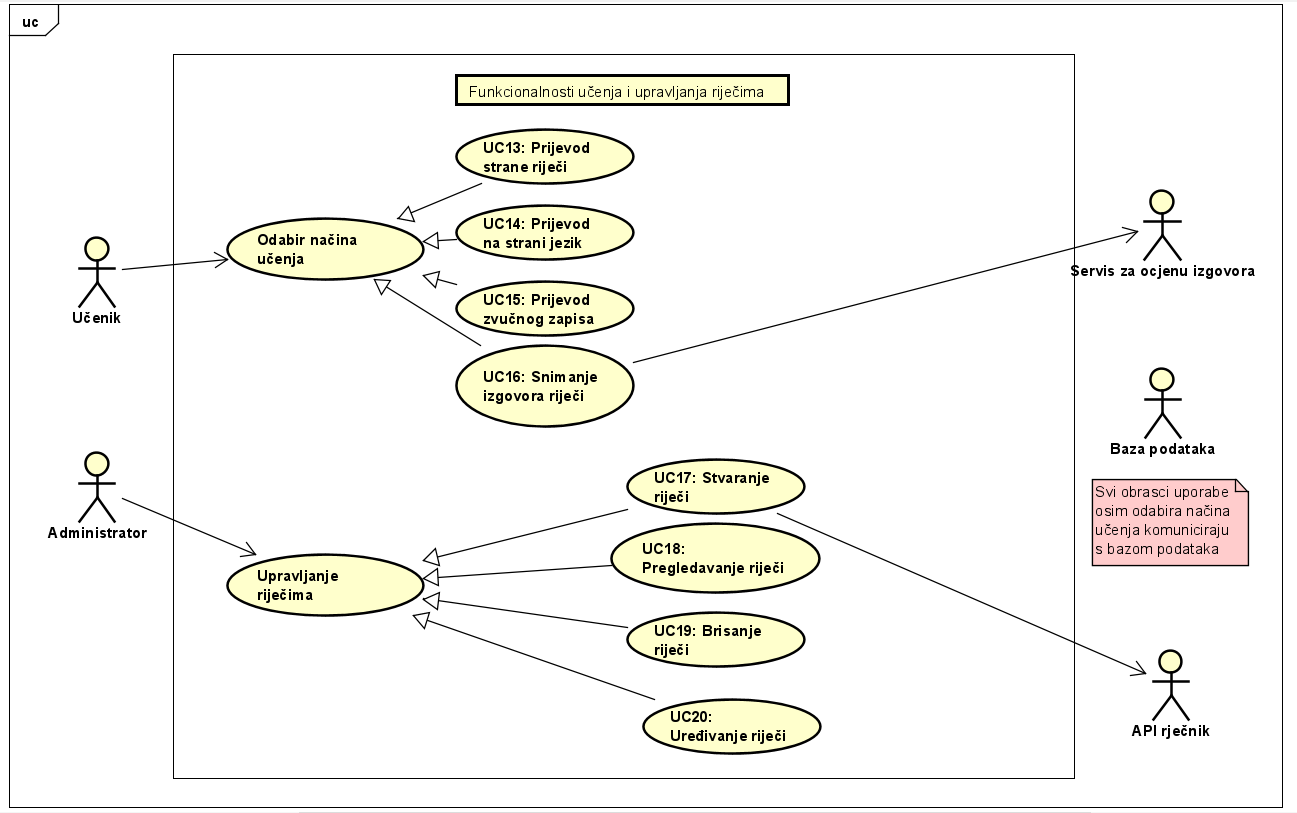
\includegraphics[scale=0.6]{dijagrami/upravljanje_rijecima.png} 
	\centering
	\caption{Funkcionalnosti učenja i upravljanja riječima}
	\label{fig:dijagram1}
\end{figure}

\begin{figure}[H]
	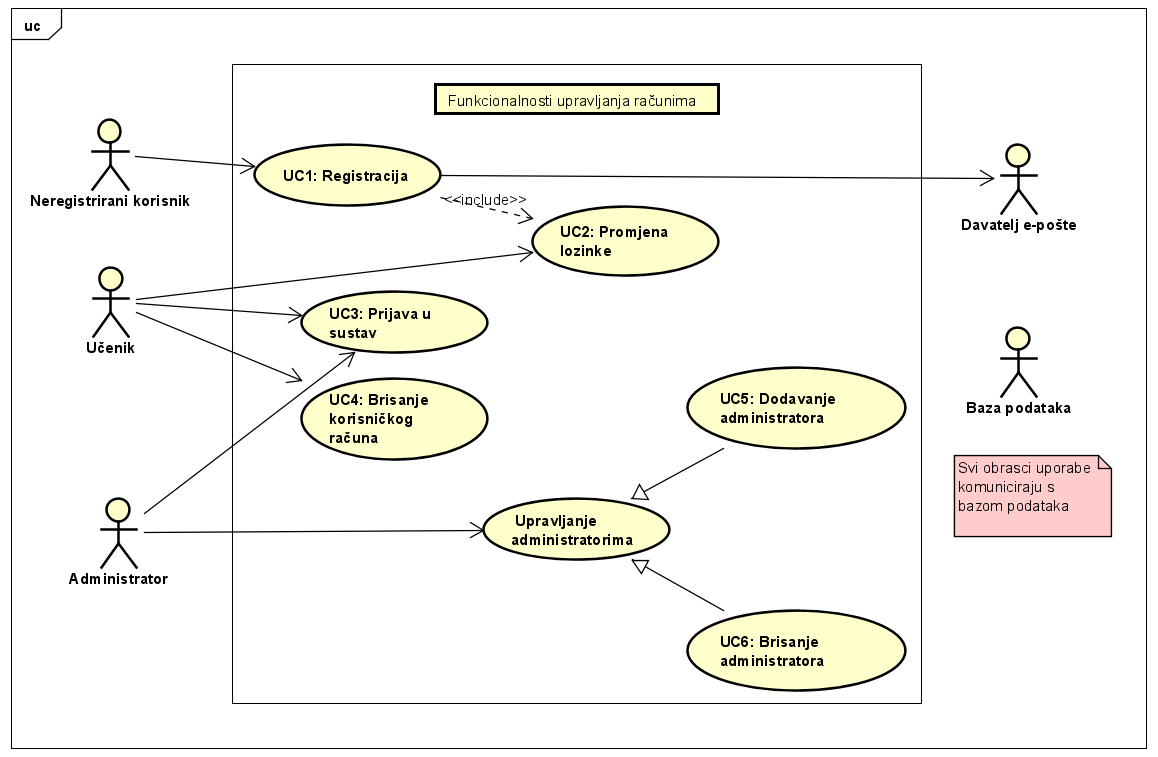
\includegraphics[scale=0.6]{dijagrami/upravljanje_Racunima.png} 
	\centering
	\caption{Funkcionalnosti upravljanja računima}
	\label{fig:dijagram2}
\end{figure}

\begin{figure}[H]
	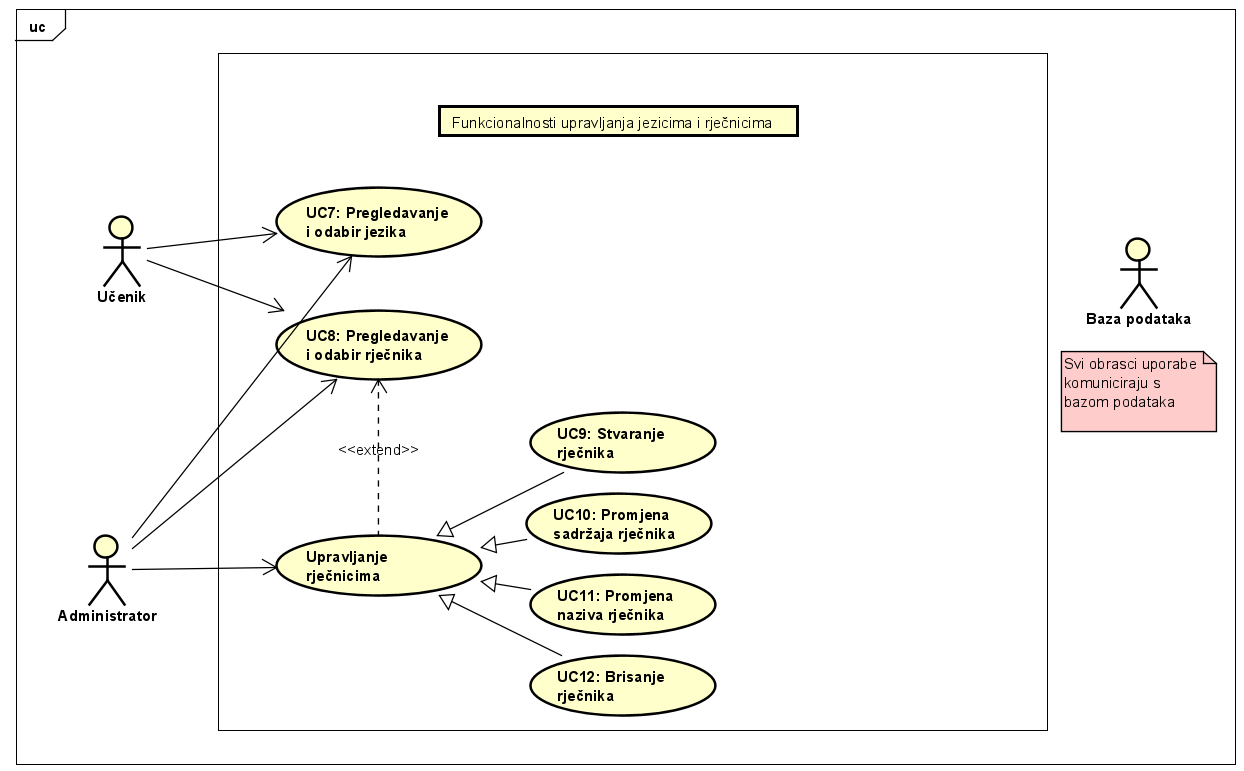
\includegraphics[scale=0.6]{dijagrami/upravljanje_rjecnicima.png} 
	\centering
	\caption{Funkcionalnosti upravljanja jezicima i rječnicima}
	\label{fig:dijagram3}
\end{figure}	

\subsection{Sekvencijski dijagrami}

\subsubsection{{Obrazac uporabe 1: Registracija}}


Neregistrirani korisnik započinje registraciju odabirom opcije "Registracija" na korisničkom sučelju. Nakon što je opcija odabrana, poslužitelj šalje zahtjev korisniku da unese svoje osobne podatke, uključujući ime, prezime i e-mail adresu. Korisnik unosi tražene podatke i nakon toga potvrđuje svoju registraciju putem korisničkog sučelja. Poslužitelj započinje proces provjere unesenih podataka. Prvo, provjerava dostupnost e-mail adrese u bazi podataka kako bi utvrdio postoje li odstupanja. U slučaju da e-mail adresa već postoji u bazi podataka ili nije ispravna, poslužitelj obavještava korisnika o nemogućnosti registracije i sprječava daljnji napredak u procesu. Ukoliko su svi uneseni podaci ispravni, poslužitelj generira privremenu lozinku za korisnika, koja se šalje na njegovu e-mail adresu. Nakon što korisnik primi privremenu lozinku putem e-maila, on se prijavljuje u sustav koristeći svoje korisničko ime (e-mail adresu) i privremenu lozinku. Odmah nakon uspješne prijave, korisniku se prikazuje obrazac za promjenu inicijalne lozinke. Korisnik unosi novu lozinku koju želi koristiti za pristup sustavu i poslužitelj ažurira podatke u bazi.

\begin{figure}[htp]
	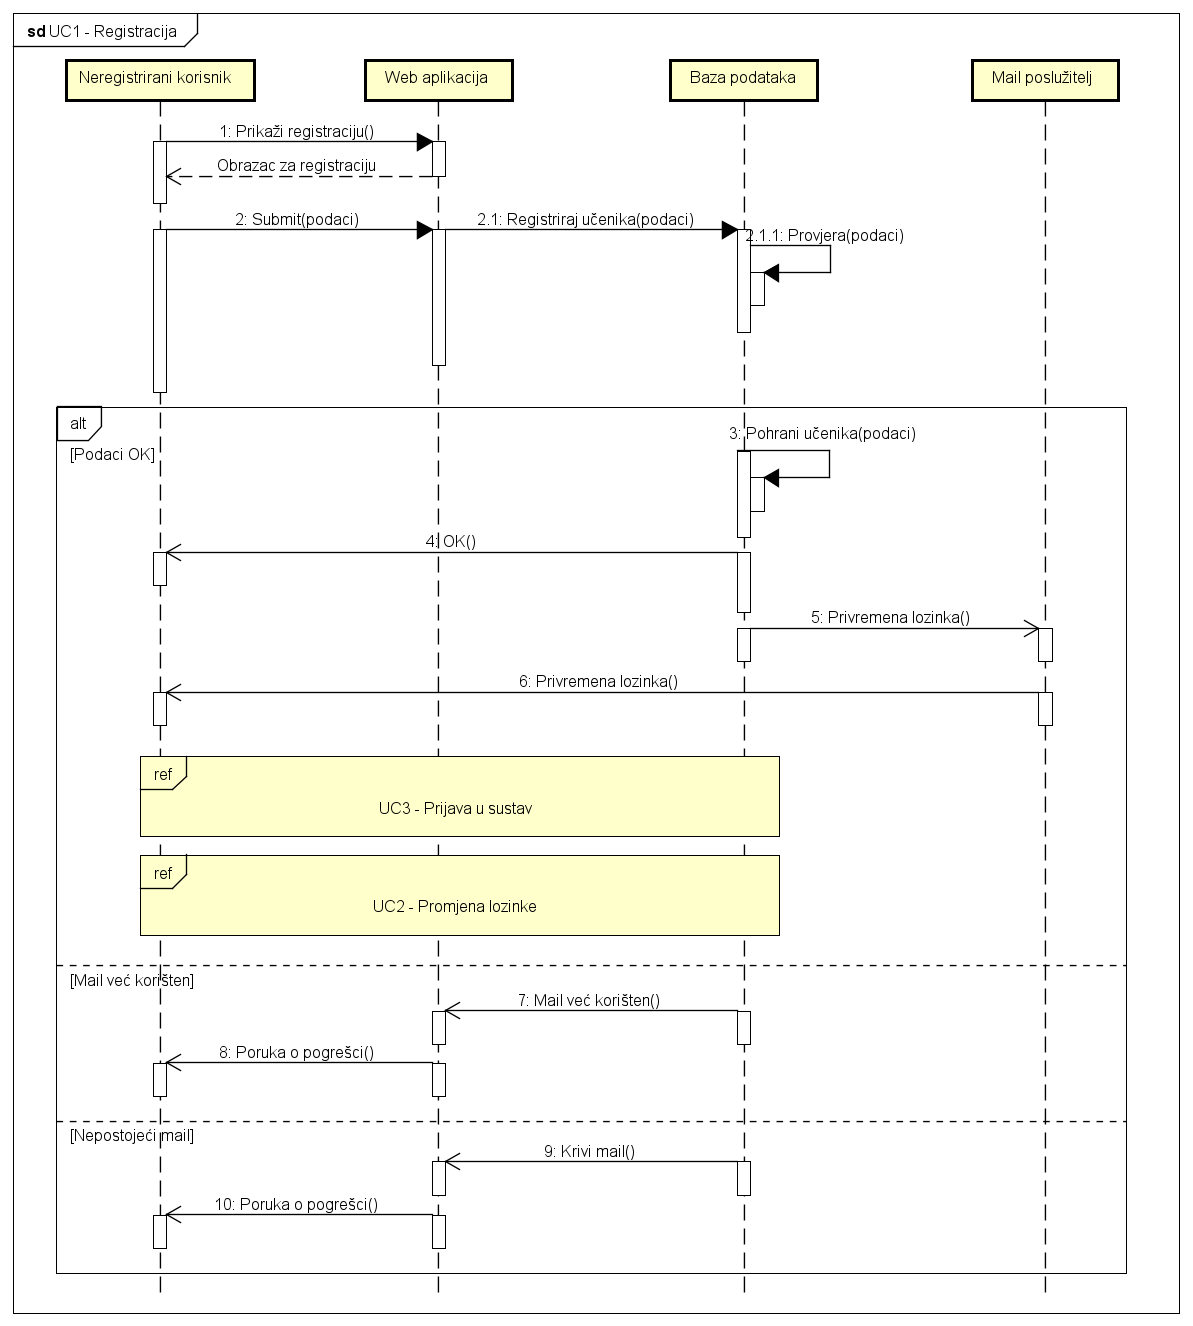
\includegraphics[scale=0.45]{dijagrami/UC1 - Registracija.png}
	\centering
	\caption{Sekvencijski dijagram, UC1 Registracija}
	\label{fig:uc-registracija}
\end{figure}

\eject

\subsubsection{{Obrazac uporabe 8 -- Pregledavanje i odabir rječnika}}

Nakon što je odabrao jezik, korisniku se treba prikazati popis svih dostupnih rječnika za taj jezik, a web aplikacija te podatke dohvaća slanjem upita na bazu podataka. Prije prikazivanja podataka korisniku, web aplikacija provjerava koliko je rječnika vratila baza. U slučaju da baza nije vratila nijedan rječnik, korisniku se prikazuje poruka da za odabrani jezik trenutno ne postoji nijedan rječnik. Inače se korisniku prikazuje popis rječnika.

I administratori i učenici mogu pristupati odabiru rječnika. Odabirom rječnika web aplikacija preusmjerava učenika na zaslon za odabir načina učenja, dok administratora preusmjerava na zaslon sa detaljnijim sadržajem rječnika (popisom riječi u rječniku, nazivom rječnika). U slučaju da administrator ne odabere rječnik, već zatraži brisanje rječnika, web aplikacija mu prikazuje okvir za potvrdu brisanja rječnika preko kojeg može izbrisati rječnik iz sustava. Administrator također može odabrati opciju za stvaranje novog rječnika, nakon čega ga web aplikacija preusmjerava na zaslon s obrascem za stvaranje rječnika.

\begin{figure}[p]
	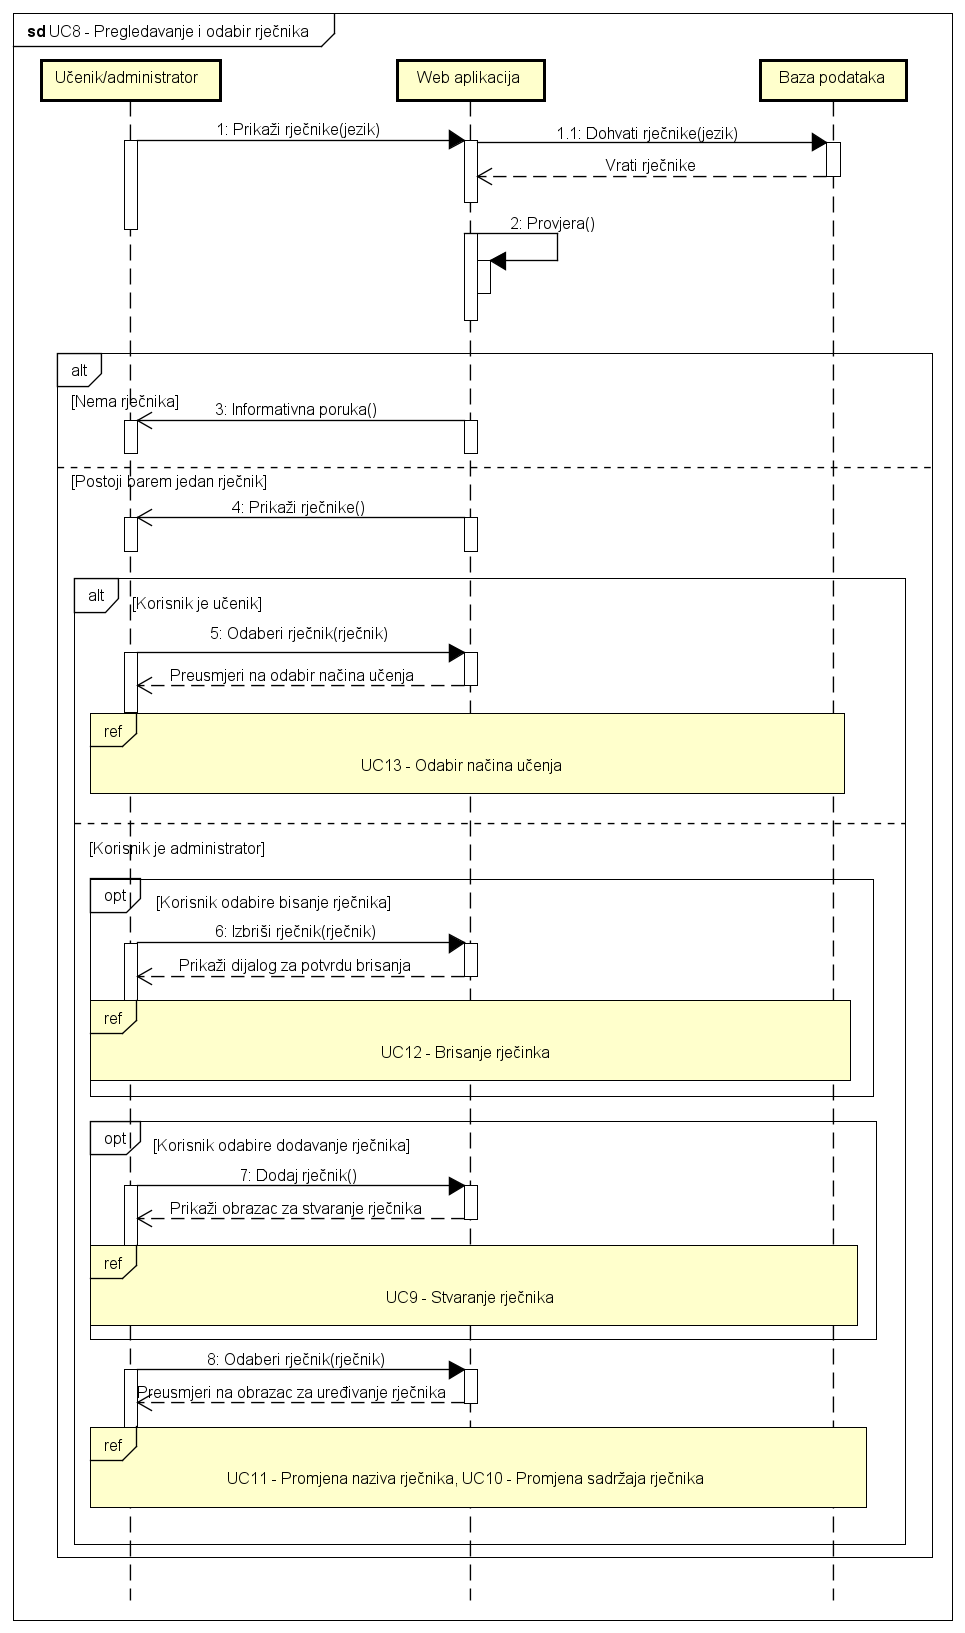
\includegraphics[scale=0.5]{dijagrami/UC8 - Pregledavanje i odabir rječnika.png}
	\centering
	\caption{Sekvencijski dijagram, UC8 Pregledavanje i odabir rječnika}
	\label{fig:uc-odabir-rjecnika}
\end{figure}

\eject

\subsubsection{{Obrazac uporabe 10 - Promjena sadržaja rječnika}}

Administrator šalje zahtjev web aplikaciji za popis svih riječi u rječniku. Web aplikacija dohvaća popis riječi iz baze podataka te ga prikazuje korisniku. Ako administrator odabere opciju "ukloni" pored određene riječi, tada šalje zahtjev za uklanjanje aplikaciji, a aplikacija šalje zahtjev za brisanje riječi u bazi podataka i potvrđuje brisanje administratoru. U slučaju da administrator odabere opciju "dodaj riječ", aplikacija dohvaća riječi koje se ne nalaze u rječniku iz baze podataka i prikazuje ih administratoru. Ako nema dostupnih riječi, aplikacija šalje informativnu poruku administratoru umjesto popisa. U suprotnom, administrator odabire jednu ili više riječi, potvrđuje odabir, i riječi se pohranjuju u bazu podataka putem aplikacije.

\begin{figure}[p]
	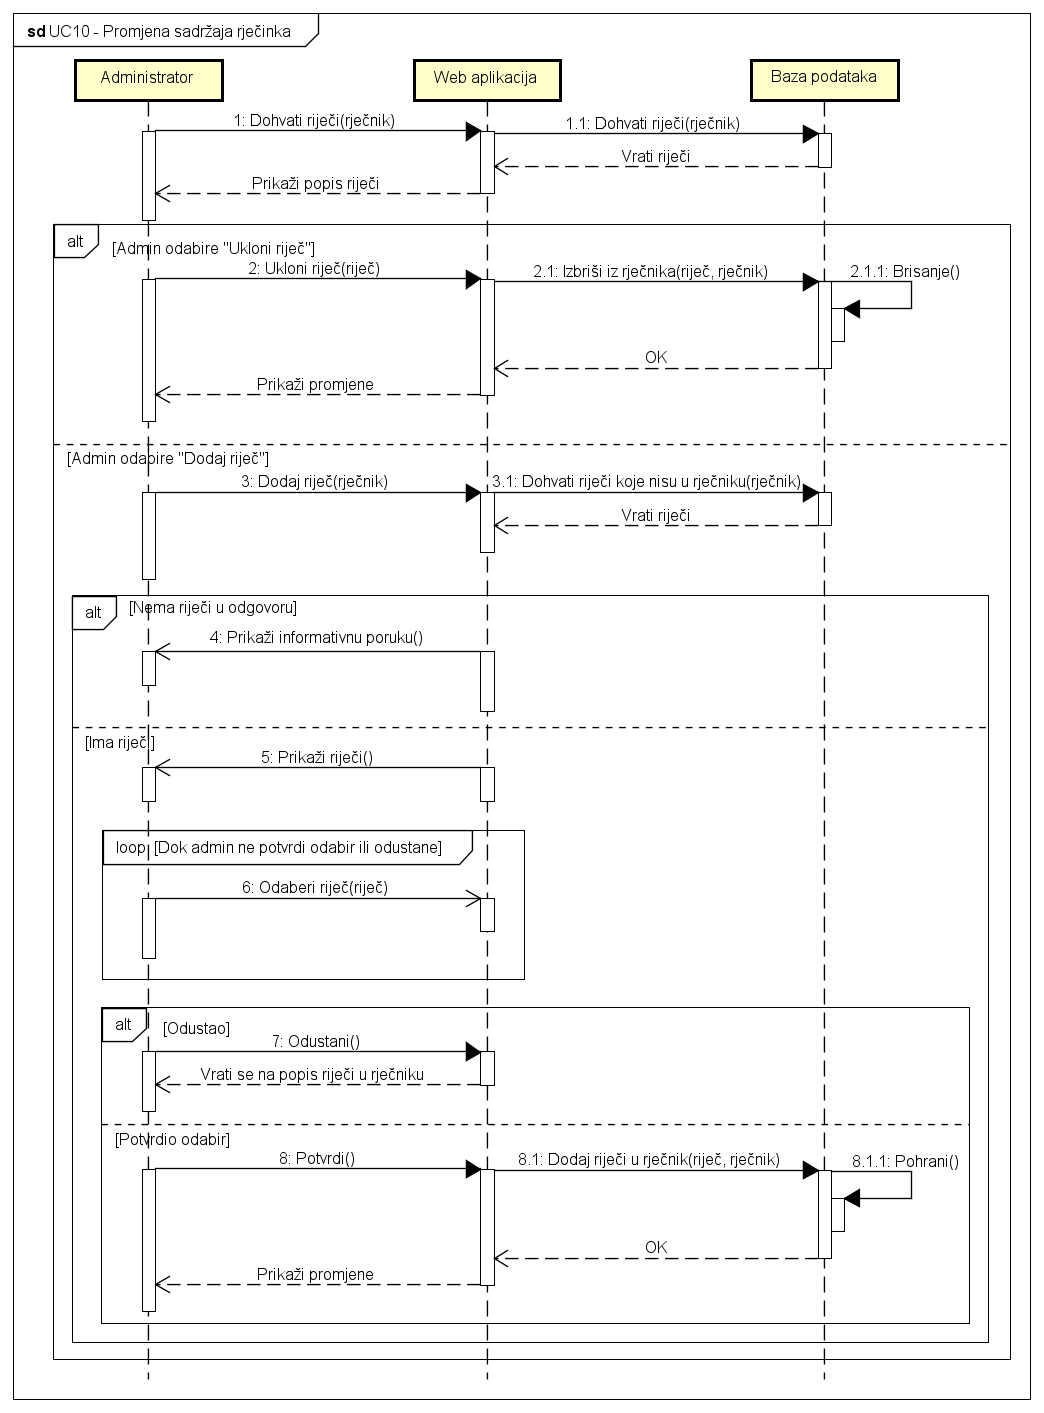
\includegraphics[scale=0.55]{dijagrami/UC10 - Promjena sadržaja rječinka.png}
	\centering
	\caption{Sekvencijski dijagram, UC10 Promjena sadržaja rječnika}
	\label{fig:uc-promjena-rjecnika}
\end{figure}

\eject

\section{Ostali zahtjevi}

\begin{itemize}
\item sustav korisniku daje povratnu informaciju o točnosti njegova odgovora
\item sustav u razumnom vremenu prezentira riječi nakon odabira načina rada
\item sustav mora imati potporu hrvatskih dijakritičkih znakova
\item sustavu iz javne mreže pristupamo protokolom HTTPS
\item sustav je dovoljno jednostavan i intuitivan za bilo koju dobnu skupinu korisnika 
\item za korištenje sustava korisniku je potrebno poznavanje hrvatskog jezika
\item prijevodi riječi moraju biti ispravni
\end{itemize}
